\documentclass{beamer}

\usepackage[utf8]{inputenc}
\usepackage{tikz}
\usepackage[ruled, linesnumbered]{algorithm2e}

\title{Introduction to Multilayer Perceptron}
\subtitle{Multilayer Fully Connected Feedforward Neural Networks}
\author{Vitor Greati\inst{1}}
\institute[]
{
	\inst{1}%
	Federal University of Rio Grande do Norte
}
\date{}
\subject{Computer Science}

% Table of contents at the beginning of each section
\AtBeginSection[]
{
  \begin{frame}
    \frametitle{Table of Contents}
    \tableofcontents[currentsection]
  \end{frame}
}

% Table of contents at the beginning of each subsection
%\AtBeginSubsection[]
%{
%  \begin{frame}
%    \frametitle{Table of Contents}
%    \tableofcontents[currentsection,currentsubsection]
%  \end{frame}
%}

\begin{document}

\frame{\titlepage}

\section{Introduction}

    \subsection{Concept}

         \begin{frame}{Concept}{Defining Neural Networks}

            Neural Networks or Artificial Neural Networks are computational models
            inspired in the neural system, containing a \textbf{labelled directed graph} $G=(V,E)$ whose nodes 
            are capable of performing some \textbf{simple computation} and where each edge $(u,v) \in E$ \textbf{carries the output}
            of such computation from $u$ to $v$ increased or diminished by the \textbf{edge weight} $w(u,v)$.\\~\\ 

The weights
            indicate the importance degree of the signal of each connection.\\~\\

In a Neural Network,
            these \textbf{weights are modified} during the learning process by \textbf{learning algorithms}.

        \end{frame}

    \subsection{Applications}
        \begin{frame}{Applications}{Neural Networks for what?}

            Neural networks can be applied to supervised, unsupervised and semi-supervised learning
            tasks, given the right architecture.\\~\\

            Common applications are:
            \begin{itemize}
                \item classification;
                \item regression;
                \item clustering;
                \item vector quantization;
                \item pattern association;
                \item function approximation.
            \end{itemize}
        \end{frame}

    \subsection{Neurons}
    \begin{frame}{Neurons}{Basic elements}

        The neuron's basic task is to take an input, perform some computation and
        output a value.

        \begin{block}{Main elements}
            \begin{itemize}
                \item An input vector $\mathbf{x} = \langle x_1, x_2, \ldots, x_n \rangle \in \mathbb{R}^n$.
                \item A vector of weights $\mathbf{w} = \langle w_1, w_2, \ldots, w_n \rangle \in \mathbb{R}^n$.
                \item A value $b \in \mathbb{R}$, called \emph{bias}.
                \item A computation between inputs and weights, like 
                    $$z=\mathbf{x}\cdot\mathbf{w} =\sum_i x_iw_i.$$
                \item An activation function $f$ to produce an output $f(z + b)$.
            \end{itemize}
        \end{block}
    \end{frame}

    \begin{frame}{Neurons}{Graphical representation}
        A common graphical representation highlights those elements:
        \begin{figure}
            \centering
            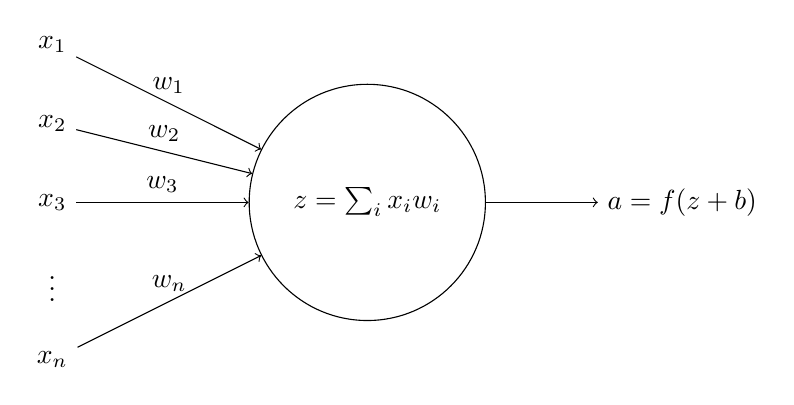
\begin{tikzpicture}
                \draw (4,1) node[circle,minimum size=3cm,draw] (A) {};
                \node (B) at (0,3) {$x_1$};
                \node (C) at (0,2) {$x_2$};
                \node (D) at (0,1) {$x_3$};
                \node (E) at (0,0) {$\vdots$};
                \node (F) at (0,-1) {$x_n$};
                \draw [->] (B) -- node [above] {$w_1$} (A);
                \draw [->] (C) -- node [above] {$w_2$}(A);
                \draw [->] (D) -- node [above] {$w_3$}(A);
                \draw [->] (F) -- node [above] {$w_n$}(A);
                \node (H) at (8,1) {$a=f(z+b)$};
                \draw [->] (A) -- (H);
                \node (G) at (4,1) {$z=\sum_i x_iw_i$};
            \end{tikzpicture}
        \end{figure}
    \end{frame}

    \begin{frame}{Neurons}{Graphical representation}
        The same representation, but using only vectors:

        \begin{figure}
            \centering
            \begin{tikzpicture}
                \draw (4,1) node[circle,minimum size=3cm,draw] (A) {};
                \node (D) at (0,1) {$\mathbf x$};
                \draw [->] (D) -- node [above] {$\mathbf w$}(A);
                \node (H) at (8,1) {$a=f(z+b)$};
                \draw [->] (A) -- (H);
                \node (G) at (4,1) {$z=\mathbf{x} \cdot \mathbf{w}$};
            \end{tikzpicture}
        \end{figure}
    \end{frame}

    \subsection{Activation functions}

        \begin{frame}{Activation functions}{Sigmoid function}
            
            The sigmoid is a classical function in the neuron activation context. It is defined by:

            \begin{displaymath}
                f_{sig}(net) = \frac{1}{1 + e^{-net}}
            \end{displaymath}

            When compared to the step function:
            \begin{itemize}
                \item $f_{sig}$ is continuous and differentiable everywhere;
                \item $f_{sig}$ is symmetric around the y-axis;
                \item $f_{sig}$ asymptotically approaches its saturation values.
            \end{itemize}

            However:
            \begin{itemize}
                \item $f_{sig}$ outputs are not zero centered;
                \item Saturated neurons essentially kill the gradient, since the delta will be extremely small.
            \end{itemize}
        \end{frame}


        \begin{frame}{Activation functions}{Step function}

            The step function is defined as
            \begin{displaymath}
                f_s(net) = 
                \begin{cases}
                    1, net > 0\\
                    0, net < 0\\
                \end{cases}
            \end{displaymath}

            Notice that:
            \begin{itemize}
                \item $f_s$ only lets the signal pass if the computation results in a positive net;
                \item $f_s$ is not differentiable, which produce problems for some learning algorithms; 
            \end{itemize}

            This activation is used in the classic \textbf{Perceptron}.

        \end{frame}


        \begin{frame}{Activation functions}{Hyperbolic tangent function}

            The hyperbolic tangent function is defined as
            \begin{displaymath}
                f_{tanh}(net) = \tanh(net) = \frac{e^{net} - e^{-net}}{e^{net} + e^{-net}}.
            \end{displaymath}

            Notice that:
            \begin{itemize}
                \item $f_{tanh}$ is zero centered;
                \item The problem for saturated neurons remains.
            \end{itemize}

        \end{frame}

        \begin{frame}{Activation functions}{ReLU - Rectified Linear Unit}

            The ReLU function is defined as:

            \begin{displaymath}
                f_{relu}(net) = \max(0, net).
            \end{displaymath}

            Notice:
            \begin{itemize}
                \item $f_{relu}$ is not saturable and it is extremely efficient;
                \item $f_{relu}$ is not differentiable at $0$.
            \end{itemize}

        \end{frame}

        \begin{frame}{Activation functions}{Leaky ReLU - Leaky Rectified Linear Unit}
            The Leaky ReLU is defined as:

            \begin{displaymath}
                f_{lrelu}(net)=
                \begin{cases}
                    net, net \geq 0\\
                    \alpha \times net, net < 0
                \end{cases}
            \end{displaymath}

            \begin{itemize}
                \item $f_{lrelu}$ allows a small, non-zero gradient at $0$;
                \item $f_{lrelu}$ allows negative values;
                \item PReLUs, Parametric ReLUs, allows $\alpha$ to be learned differently for each node.
            \end{itemize}
        \end{frame}

        \begin{frame}{Activation functions}{ELU - Exponential Linear Units}
            The ELU function is defined as:

            \begin{displaymath}
                f_{elu}(net) = 
                \begin{cases}
                    net, net \geq 0\\
                    \alpha \times (e^{net} - 1), neq < 0
                \end{cases}
            \end{displaymath}

            Here, $\alpha$ is a constant, set when the network is instantiated. A common
            value for it is $\alpha = 1.0$.\\~\\

            ELUs have presented better results than ReLUs.

        \end{frame}



\section{Multilayer Perceptron}

    \subsection{Architecture}

        \begin{frame}{Multilayer Architecture}{Fully connected feedforward architecture}
            
            An architecture with $C$ layers, $L_0, L_1, \ldots, L_{C-1}$,
            is graphically represented as:

            \begin{figure}
                \centering
                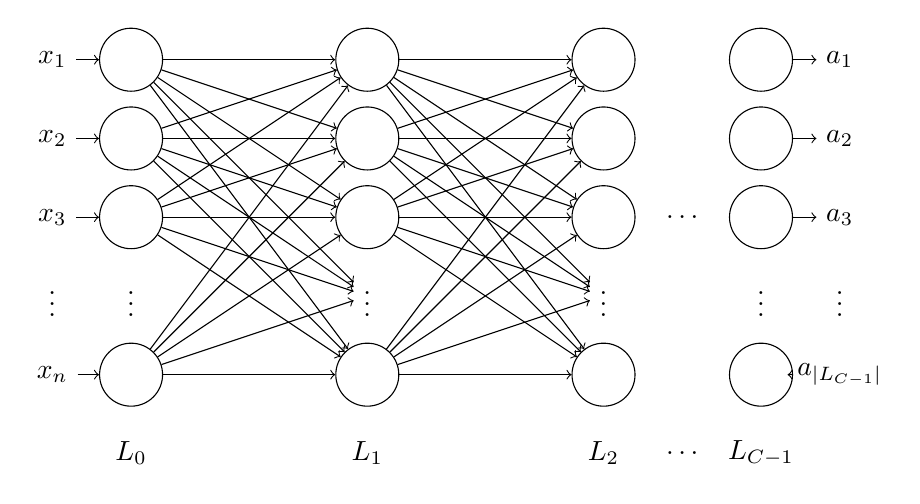
\begin{tikzpicture}
                    % Layer 1
                    \draw (0,4) node[circle,minimum size=0.8cm,draw] (A1) {};
                    \draw (0,3) node[circle,minimum size=0.8cm,draw] (A2) {};
                    \draw (0,2) node[circle,minimum size=0.8cm,draw] (A3) {};
                    \node (A) at (0,1) {$\vdots$};
                    \draw (0,0) node[circle,minimum size=0.8cm,draw] (A4) {};
                    \node (AL) at (0,-1) {$L_0$};
                    % Ins
                    \node (I1) at (-1,4) {$x_1$};
                    \draw [->](I1) -- (A1);
                    \node (I2) at (-1,3) {$x_2$};
                    \draw [->](I2) -- (A2);
                    \node (I3) at (-1,2) {$x_3$};
                    \draw [->](I3) -- (A3);
                    \node (I) at (-1,1) {$\vdots$};
                    \node (I4) at (-1,0) {$x_n$};
                    \draw [->](I4) -- (A4);
                    % Layer 2
                    \draw (3,4) node[circle,minimum size=0.8cm,draw] (B1) {};
                    \draw (3,3) node[circle,minimum size=0.8cm,draw] (B2) {};
                    \draw (3,2) node[circle,minimum size=0.8cm,draw] (B3) {};
                    \node (B) at (3,1) {$\vdots$};
                    \draw (3,0) node[circle,minimum size=0.8cm,draw] (B4) {};
                    \node (BL) at (3,-1) {$L_1$};
                    % Layer 3
                    \draw (6,4) node[circle,minimum size=0.8cm,draw] (C1) {};
                    \draw (6,3) node[circle,minimum size=0.8cm,draw] (C2) {};
                    \draw (6,2) node[circle,minimum size=0.8cm,draw] (C3) {};
                    \node (C) at (6,1) {$\vdots$};
                    \draw (6,0) node[circle,minimum size=0.8cm,draw] (C4) {};
                    \node (CL) at (6,-1) {$L_2$};
                    % Layers 4..k-1
                    \node (DDD1) at (7,2) {$\ldots$};
                    \node (DDD2) at (7,-1) {$\ldots$};
                    % Layer k
                    \draw (8,4) node[circle,minimum size=0.8cm,draw] (D1) {};
                    \draw (8,3) node[circle,minimum size=0.8cm,draw] (D2) {};
                    \draw (8,2) node[circle,minimum size=0.8cm,draw] (D3) {};
                    \node (D) at (8,1) {$\vdots$};
                    \draw (8,0) node[circle,minimum size=0.8cm,draw] (D4) {};
                    \node (DL) at (8,-1) {$L_{C-1}$};
                    % Outs
                    \node (O1) at (9,4) {$a_1$};
                    \draw [->](D1) -- (O1);
                    \node (O2) at (9,3) {$a_2$};
                    \draw [->](D2) -- (O2);
                    \node (O3) at (9,2) {$a_3$};
                    \draw [->](D3) -- (O3);
                    \node (O) at (9,1) {$\vdots$};
                    \node (O4) at (9,0) {$a_{|L_{C-1}|}$};
                    \draw [->](D4) -- (O4);
                    % Links
                    \draw [->] (A1)--(B1);
                    \draw [->] (A1)--(B2);
                    \draw [->] (A1)--(B3);
                    \draw [->] (A1)--(B4);
                    \draw [->] (A1)--(B);
                    \draw [->] (A2)--(B1);
                    \draw [->] (A2)--(B2);
                    \draw [->] (A2)--(B3);
                    \draw [->] (A2)--(B4);
                    \draw [->] (A2)--(B);
                    \draw [->] (A3)--(B1);
                    \draw [->] (A3)--(B2);
                    \draw [->] (A3)--(B3);
                    \draw [->] (A3)--(B4);
                    \draw [->] (A3)--(B);
                    \draw [->] (A4)--(B1);
                    \draw [->] (A4)--(B2);
                    \draw [->] (A4)--(B3);
                    \draw [->] (A4)--(B4);
                    \draw [->] (A4)--(B);
                    \draw [->] (B1)--(C1);
                    \draw [->] (B1)--(C2);
                    \draw [->] (B1)--(C3);
                    \draw [->] (B1)--(C4);
                    \draw [->] (B1)--(C);
                    \draw [->] (B2)--(C1);
                    \draw [->] (B2)--(C2);
                    \draw [->] (B2)--(C3);
                    \draw [->] (B2)--(C4);
                    \draw [->] (B2)--(C);
                    \draw [->] (B3)--(C1);
                    \draw [->] (B3)--(C2);
                    \draw [->] (B3)--(C3);
                    \draw [->] (B3)--(C4);
                    \draw [->] (B3)--(C);
                    \draw [->] (B4)--(C1);
                    \draw [->] (B4)--(C2);
                    \draw [->] (B4)--(C3);
                    \draw [->] (B4)--(C4);
                    \draw [->] (B4)--(C);
                \end{tikzpicture}
            \end{figure}
        \end{frame}
    
        \begin{frame}{Multilayer Architecture}{Fully connected feedforward architecture}
            \begin{block}{Observations}
                \begin{itemize}
                    \item A layer $L_i$ has its own size (number of neurons) $|L_i|$.
                    \item $L_0$ is the \textbf{input layer}.
                        \begin{itemize}
                            \item Neurons in this layer are \textbf{input neurons}.
                            \item An input neuron $j$ takes the $j$-th component of the input vector.
                            \item Input neurons do not perform any computation or
                                        activation: just output the input value.
                            \item The output of $L_0$ is $\mathbf{x}$, the input vector.
                        \end{itemize}
                    \item $L_{C-1}$ is the \textbf{output layer} and its output is the
                        network output.
                    \item Any other layer is a \textbf{hidden layer}.
                    \item This architecture is \textbf{fully connected} because each neuron in
                        layer $L_i$ is connected to every neuron in layer $L_{i+1}$.
                    \item This architecture is \textbf{feedforward} because there is no back 
                        arrows forming cycles; otherwise, it would be \emph{recurrent}.
                \end{itemize}
            \end{block}
        \end{frame}

    \subsection{Mathematical representation}
        \begin{frame}{Multilayer Architecture}{Fully connected feedforward architecture}
            How can we perform calculations and learning in this architecture? Mathematics, of course.

            \begin{block}{Representing connections between layers}
                Consider layer $L_l, l = 1, \ldots, C-1$, and neuron $k$
                of $L_l$. Since the architecture is fully connected,
                $k$ is connected to all neurons $j$ in $L_{l-1}$. 
                Denote by $w^l_{kj}$ the weight of the connection
                between neuron $j$ of $L_{l-1}$ and neuron $k$ of $L_l$:

                \begin{figure}
                    \centering
                    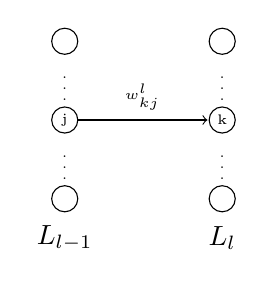
\begin{tikzpicture}
                        % Layer l-1
                        \draw (0,4) node[circle,minimum size=0.2cm,draw] (A1) {};
                        %\draw (0,3.5) node[circle,minimum size=0.2cm,draw] (A2) {};
                        \node (A) at (0,3.5) {$\tiny \vdots$};
                        \draw (0,3) node[circle,minimum size=0.2cm,draw] (A3) {};
                        \node (A) at (0,2.5) {$\tiny \vdots$};
                        \draw (0,2) node[circle,minimum size=0.2cm,draw] (A4) {};
                        \node (TLM1) at (0,3) {\tiny j};
                        \node (AL) at (0,1.5) {$L_{l-1}$};
                        % Layer l
                        \draw (2,4) node[circle,minimum size=0.2cm,draw] (A1) {};
                        %\draw (2,3.5) node[circle,minimum size=0.2cm,draw] (A2) {};
                        \draw (2,3) node[circle,minimum size=0.2cm,draw] (A3) {};
                        \node (A) at (2,3.5) {\tiny $\vdots$};
                        \node (TL1) at (2,3) {\tiny k};
                        \node (A) at (2,2.5) {\tiny $\vdots$};
                        \draw (2,2) node[circle,minimum size=0.2cm,draw] (A4) {};
                        \node (AL) at (2,1.5) {$L_{l}$};
                        % link
                        \draw [->] (TLM1) -- node [above] {\tiny $w^l_{kj}$} (TL1);
                    \end{tikzpicture}
                \end{figure}

            \end{block}

        \end{frame}


        \begin{frame}{Multilayer Architecture}{Fully connected feedforward architecture}
                In this way, we can represent all weights between two layers
                using only one matrix $\mathbf{W}^l = (w^l_{kj})$:
        
                \[
                    \mathbf{W}^l = 
                    \begin{bmatrix}
                        w^l_{11} & w^l_{12} & \ldots & w^l_{1|L_{l-1}|}\\
                        w^l_{21} & w^l_{22} & \ldots & w^l_{2|L_{l-1}|}\\
                        \vdots & \vdots & \ddots & \vdots\\
                        w^l_{|L_l|1} & w^l_{|L_l|2} & \ldots & w^l_{|L_l||L_{l-1}|}\\
                    \end{bmatrix}.
                \]                

                Notice that: 
                \begin{itemize}
                    \item $\mathbf{W}^l$ has dimensions $|L_l| \times |L_{l-1}|$.
                    \item The weight vector of connections to neuron $k$ in $L_l$ is the $k$-th row of $\mathbf{W}^l$, denoted by $\mathbf{w^l_k}$.
                    \item All connections in the network are represented! They are all in matrices $\mathbf{W}^1, \mathbf{W}^2, \ldots, \mathbf{W}^{C-1}$.
                \end{itemize}
        \end{frame}

        \begin{frame}{Multilayer Architecture}{Fully connected feedforward architecture}
            \begin{block}{Representing the biases}
                Remember that each neuron has its own bias. So, let $b^l_k$ denote the
                bias of neuron $k$ in layer $L_l$. Then, the biases in layer $l$ are 
                represented as just a vector 

                $$\mathbf{b}^l = \langle b^l_1, b^l_2, \ldots, b^l_{|L_{l}|} \rangle.$$
                
                In this way, all biases are represented by vectors $\mathbf{b}^1, \mathbf{b}^2, \ldots, \mathbf{b}^{C-1}.$
            \end{block}
        \end{frame}

        \begin{frame}{Multilayer Architecture}{Fully connected feedforward architecture}
            \begin{block}{Representing layer outputs}
                Denote by $a^l_k$ the output of neuron $k$ in layer $L_l$, and by $\mathbf{a^l}$ the output vector
                for layer $L_l$. How to compute such output? First, look: \\~\\

                \begin{figure}
                    \centering
                    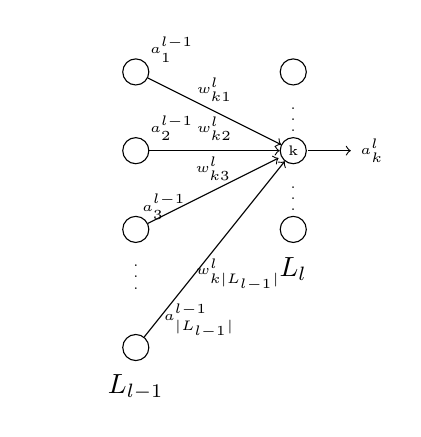
\begin{tikzpicture}
                        % Layer l-1
                        \draw (0,4) node[circle,minimum size=0.2cm,draw] (A1) {};
                        \draw (0,3) node[circle,minimum size=0.2cm,draw] (A2) {};
                        \draw (0,2) node[circle,minimum size=0.2cm,draw] (A3) {};
                        \node (A) at (0,1.5) {$\tiny \vdots$};
                        \draw (0,0.5) node[circle,minimum size=0.2cm,draw] (A4) {};
                        \node (BL) at (0,0) {$L_{l-1}$};
                        % Layer l
                        \draw (2,4) node[circle,minimum size=0.2cm,draw] (B1) {};
                        %\draw (2,3.5) node[circle,minimum size=0.2cm,draw] (A2) {};
                        \draw (2,3) node[circle,minimum size=0.2cm,draw] (B3) {};
                        \node (A) at (2,3.5) {\tiny $\vdots$};
                        \node (TL1) at (2,3) {\tiny k};
                        \node (B) at (2,2.5) {\tiny $\vdots$};
                        \draw (2,2) node[circle,minimum size=0.2cm,draw] (B4) {};
                        \node (AL) at (2,1.5) {$L_{l}$};
                        % link
                        \draw [->] (A1) node [above] {\hspace{0.8cm} \tiny $a^{l-1}_1$} -- node [above] {\tiny $w^l_{k1}$} (B3);
                        \draw [->] (A2)  node [above] {\hspace{0.8cm} \tiny $a^{l-1}_2$}-- node [above] {\tiny $w^l_{k2}$} (B3);
                        \draw [->] (A3)  node [above] {\hspace{0.6cm} \tiny $a^{l-1}_3$}-- node [above] {\tiny $w^l_{k3}$} (TL1);
                        \draw [->] (A4)  node [above] {\hspace{1.5cm} \tiny $a^{l-1}_{|L_{l-1}|}$}-- node [below] {\hspace{.6cm}\tiny $w^l_{k|L_{l-1}|}$} (B3);
                        % outs
                        \node (O1) at (3,3) {\tiny $a^l_k$};
                        \draw [->](TL1) -- (O1);
                        
                    \end{tikzpicture}
                \end{figure}
            \end{block}
        \end{frame}

        \begin{frame}{Multilayer Architecture}{Fully connected feedforward architecture}
                Denote by $z^l_k$
                the computation performed by the neuron, i.e:
                \[
                    z^l_k = \sum_j^{|L_{l-1}|} w^l_{kj}a^{l-1}_{j} = \mathbf{w^l_k}\mathbf{a^{l-1}}.
                \]
                Then, the neuron output is
                \[
                    a^l_k = f(z^l_k + b^l_k).
                \]
                And the \textbf{layer output} is
                \[
                    \mathbf{a}^l = \mathbf{f}(\mathbf{W}^l \cdot \mathbf{a}^{l-1} + \mathbf{b}^l).
                \]
        \end{frame}

        \begin{frame}{Multilayer Architecture}{Fully connected feedforward architecture}
                Didn't get it? Look: 

                {\tiny
                \begin{align*}
                    \mathbf{f}\left( \mathbf{W}^l \cdot \mathbf{a^{l-1}} + \mathbf{b^l} \right) &=
                    \mathbf{f} \left( \begin{bmatrix}
                        w^l_{11} & w^l_{12} & \ldots & w^l_{1|L_{l-1}|}\\
                        w^l_{21} & w^l_{22} & \ldots & w^l_{2|L_{l-1}|}\\
                        \vdots & \vdots & \ddots & \vdots\\
                        w^l_{|L_l|1} & w^l_{|L_l|2} & \ldots & w^l_{|L_l||L_{l-1}|}\\
                    \end{bmatrix}
                    \cdot
                    \begin{bmatrix}
                        a^{l-1}_1 \\ a^{l-1}_2  \\ \vdots  \\ a^{l-1}_{|L_{l-1}|}
                    \end{bmatrix}
                    +
                    \begin{bmatrix}
                        b^{l}_1 \\ b^{l}_2  \\ \vdots  \\ b^{l}_{|L_l|}
                    \end{bmatrix}
                    \right)\\
                    & =
                    \mathbf{f}\left( \begin{bmatrix}
                        \sum_j^{|L_{l-1}|} w_{1j}a^{l-1}_j + b^l_1\\
                        \sum_j^{|L_{l-1}|} w_{2j}a^{l-1}_j + b^l_2\\
                        \vdots\\
                        \sum_j^{|L_{l-1}|} w_{|L_l|j}a^{l-1}_j + b^l_{|L_l|}\\
                    \end{bmatrix} \right)\\
                    & = 
                    \mathbf{f} \left( \begin{bmatrix}
                        \mathbf{w^l_1}\mathbf{a^{l-1}} + b^l_1\\
                        \mathbf{w^l_2}\mathbf{a^{l-1}} + b^l_2\\
                        \vdots\\
                        \mathbf{w^l_{|L_l|}}\mathbf{a^{l-1}} + b^l_{|L_l|}\\
                    \end{bmatrix}\right)\\
                    & = 
                    \begin{bmatrix}
                        f(z^l_1) & 
                        f(z^l_2) &
                        \ldots &
                        f(z^l_{|L_l|})
                    \end{bmatrix}^T\\
                    & =
                    \begin{bmatrix}
                        a^l_1 & 
                        a^l_2 &
                        \ldots &
                        a^l_{|L_l|}
                    \end{bmatrix}^T\\
                    & = 
                    \mathbf{a^l}
                \end{align*}
                }
        \end{frame}

    \subsection{Output computation}
        \begin{frame}{Multilayer Architecture}{Computing the network output}
            Given an input vector $\mathbf{x}$, how to compute the output of the network?\\~\\
            We have an equation to compute any $\mathbf{a}^l$ and the algorithm just goes like this:

            \begin{algorithm}[H]
                \KwIn{Input vector $\mathbf{x}$}
                \KwOut{Network output $\mathbf{a}^{C-1}$}
                \Begin{
                    $\mathbf{a}^0 \gets \mathbf{x}$\\
                    \For{$l \gets 1$ \KwTo $C-1$}{
                        $\mathbf{a}^l \gets \mathbf{W}^l \cdot \mathbf{a}^{l-1} + \mathbf{b}^l$ 
                    }
                    \Return{ $\mathbf{a}^{C-1}$}
                }
            \end{algorithm}
        \end{frame}

\end{document}
